\documentclass[border=10pt]{standalone}
\usepackage{pgfplots}
\usepgfplotslibrary{colormaps}
\pgfplotsset{trig format plots=rad}
\begin{document}
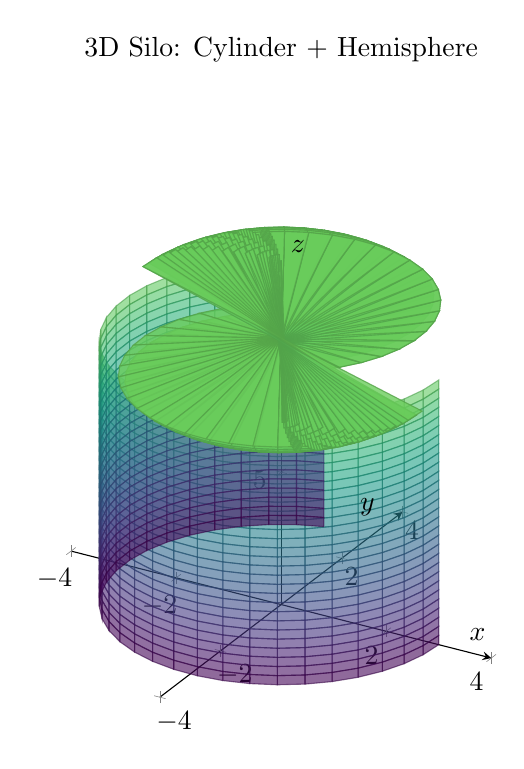
\begin{tikzpicture}
\begin{axis}[
    width=10cm, height=10cm,
    view={30}{30},
    xlabel={$x$}, ylabel={$y$}, zlabel={$z$},
    xmin=-4, xmax=4,
    ymin=-4, ymax=4,
    zmin=0, zmax=14,
    axis lines=center,
    colormap/viridis,
    title={3D Silo: Cylinder + Hemisphere}
]
% Cylinder
\addplot3[
    surf,
    domain=0:2*pi,
    y domain=0:10,
    samples=30,
    opacity=0.6
]
({3*cos(deg(x))}, {3*sin(deg(x))}, {y});

% Hemisphere
\addplot3[
    surf,
    domain=0:pi/2,
    y domain=0:2*pi,
    samples=30,
    opacity=0.8
]
({3*sin(deg(x))*cos(deg(y))}, {3*sin(deg(x))*sin(deg(y))}, {10 + 3*cos(deg(x))});

\end{axis}
\end{tikzpicture}
\end{document}
